\documentclass[a4paper,10pt,onecolumn]{article}
\usepackage{amsmath}
\usepackage{framed}
\usepackage{graphicx}

\setlength\parindent{0pt} % Remove automatical indent for new paragraph

\begin{document}

\title{Practical Programming Exam\\ Exercise 20 and question 10.3}
\author{Jonas Hjorth Knudsen\\ 201406333}
\date{\today}

\maketitle



\section{Question 3 from lecture 10*}
*NOTICE: question taken from lecture 10 since lecture 11 does not contain a question 3.\\

\textit{Suppose you run the command \emph{make main} and it fails with diagnostics}

\begin{framed}
cc \hspace{1cm} main.c \hspace{1cm} -o main\\
main.c:1:19: fatal error: gsl\_sf.h: No such file or directory\\
compilation terminated.
\end{framed}

\textit{Explain the error and how to correct it.}\\

The error occur because the header in main.c is wrong. The headerfile is \mbox{\#include\textless gsl\_sf.h\textgreater}
 when it should be \#include\textless gsl/gsl\_sf.h\textgreater.
The reason for haveing gsl/... is because the gsl library files are installed in their own directory called gsl.




\section{Exercise 20 - Numeric Arctan}

This exercise require to calculate arctan as $\arctan(x) = \int_0^x \frac{1}{x^2+1} \mathrm{d}x$.

My arctan is calculated as seen in the file \texttt{numArctan.c}. Here the integrand is defined in the function \emph{arctanInteg} and is used
in the \emph{gsl\_function} to be used in \emph{gsl\_integration\_qag} routine. To simplify the calculation I have reduced the argument in the following ways:

\begin{enumerate}
	\item if $x=0$ return $\operatorname{arctan}(x)=0$
	\item if $x<0$ return $-\operatorname{arctan}(-x)$
	\item if $x>1$ return $\frac{\pi}{2} - \operatorname{arctan}(\frac{1}{x})$
\end{enumerate}

In \texttt{main.c} a message is written to the error stream (stderr) if the result from my arctan is different from math.h's atan according to the equal method made in lecture 2 with $\mathrm{tau} = 10^{-6}$ and $\mathrm{epsilon} = 10^{-6}$. This never occur and in \texttt{outArctan.txt} the difference (error) can be seen to be maximum around $10^{-16}$. 

My solution together with math.h's atan function is plotted as seen in Figure~\ref{fig:arctan}. It can be seen that the lines lie on top of each other with follows from the low errors from the output file.

\begin{figure}[!htbp]
	\centering
	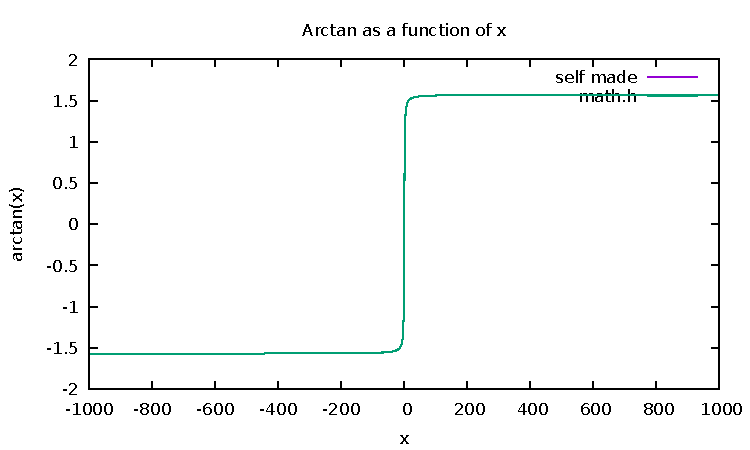
\includegraphics{plotArctan.pdf}
	\caption{Self made arctan function plotted with math.h atan function. It can be seen that the two lines lie on top of each other.}
	\label{fig:arctan}
\end{figure}


\end{document}
